\section{Introduction}
\label{sec:intro}

Networks with far more parameters than training points are easier to train than
small ones, and several accounts of this exist: a large random network contains
good sparse subnetworks \citep{frankle2019lottery,ramanujan2020hidden}; a wide
network stays close to its linearisation around the initial weights
\citep{jacot2018ntk,chizat2019lazy}; and test risk can fall again past the
interpolation threshold \citep{belkin2019reconciling,nakkiran2020double}. This
paper examines a simpler geometric picture, which we call the \emph{squiggly
line conjecture}, and reports that it does not work.

The picture is as follows. Scatter random points on a plane and draw two curves
without looking at the points, one smooth and one squiggly. The squiggly curve
passes closer to the points on average, because it visits more of the plane
(\cref{fig:two}). A network computes a function, and the graph of that function
is such a curve. The conjecture says that a network with more parameters is a
squigglier curve at initialisation, that it therefore starts closer to its
data, and that this is why it learns faster. This is a chain of three claims.

\begin{description}\setlength{\itemsep}{0pt}
\item[(G) Geometry.] A squigglier curve has a smaller mean Euclidean distance
from a data point to the nearest point of the curve.
\item[(P) Parameters.] More parameters give a squigglier random function.
\item[(L) Learning.] A smaller nearest-point distance means a smaller training
loss at initialisation.
\end{description}

\begin{figure}[t]
  \centering
  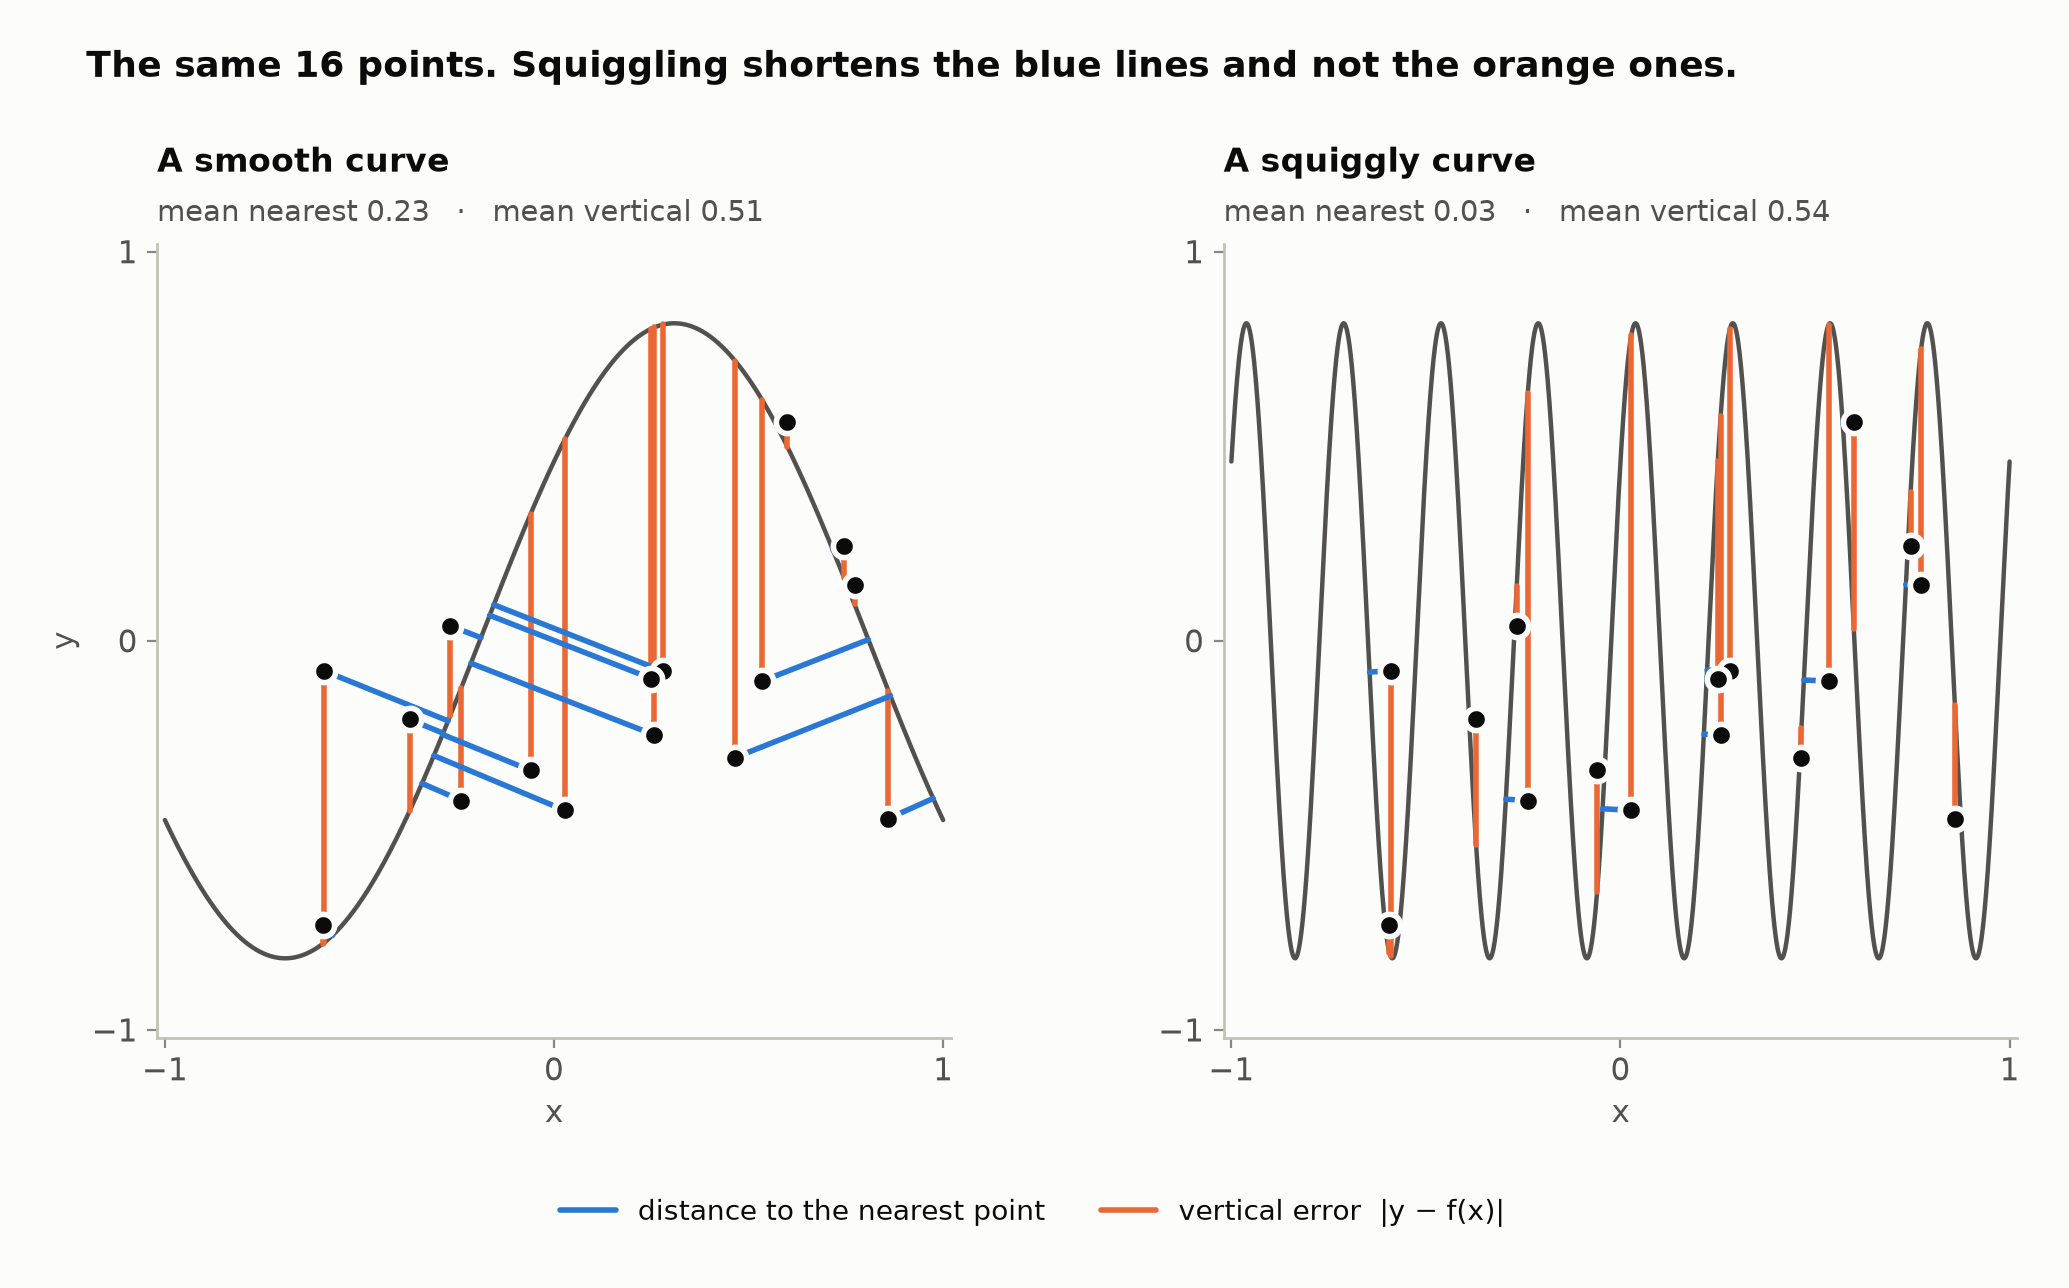
\includegraphics[width=0.78\linewidth]{../graphs/readme_two_distances.png}
  \caption{The two distances, on the same 16 points. Blue: distance to the
  nearest point of the curve. Orange: vertical error $|y-f(x)|$. Raising the
  frequency of the sine from 1 (left) to 8 (right) shortens the blue segments
  and leaves the orange ones as long as before.}
  \label{fig:two}
\end{figure}

\paragraph{Results.} (G) is true, (P) is false for width and holds weakly for
depth, and (L) is false.
\begin{itemize}\setlength{\itemsep}{0pt}
\item \emph{Slope sandwich} (\cref{thm:sandwich}). For a $K$-Lipschitz function
and any data point, $\text{vertical}/\sqrt{1+K^2}\le\text{nearest}\le\text{vertical}$.
The curve can be much nearer than its vertical error only where it is steep.
\item \emph{Marginal lemma} (\cref{thm:marginal}). The expected loss of a random
function, for any loss of the residual $y-f(x)$, depends only on the
distribution of $f(x)$ at each single $x$. For random-phase waves this
distribution does not depend on the frequency (\cref{cor:phase}), and for ReLU
networks under He initialisation the expected initial squared error does not
depend on the width (\cref{cor:he}).
\item \emph{Tube identity and length bound} (\cref{thm:tube,prop:length}). The
mean distance from a random point to a set is the mass outside the tube of
radius $r$ around the set, integrated over $r$. For a curve of length $l$ and a
uniform point in a planar region of area $V$ it is at least
$V/(4l+2\sqrt{\pi V})$.
\item \emph{The sine} (\cref{prop:sine,prop:floor}). For a sine that spans the
data, distance times frequency tends to $(2-8/\pi^2)/4\approx0.2974$. With a
smaller amplitude the distance stops at a floor set by the amplitude, not by
the number of points.
\item \emph{Experiments} (\cref{sec:experiments}). With amplitude and marginals
held fixed, the nearest-point distance falls from $0.613$ to $0.021$ while the
vertical error stays between $0.665$ and $0.669$. Random ReLU networks have the
predicted, width-independent initial squared error, and their curves are not
longer at larger width.
\end{itemize}

\paragraph{Scope.} This is a negative result about one intuitive picture. An
earlier draft of this paper claimed empirical support for the conjecture; that
support came from faulty measurement code, and the draft was withdrawn
(\cref{app:wrong}). The individual statements here are elementary, and we make
no claim of priority for any of them; \cref{sec:related} lists the work we are
aware of. \Cref{thm:sandwich,thm:marginal,thm:tube} and \cref{cor:phase} are
formalised in Lean~4 (\cref{sec:lean}). Code, the Lean project and the
development notes are at \repo.
